% This documents contain no AI writing, only my english, my phrasing, (and of course my mistakes).

\documentclass[11pt,a4paper]{article}

\usepackage[utf8]{inputenc}
\usepackage[T1]{fontenc}
\usepackage[english]{babel}
\usepackage{natbib}
\usepackage{graphicx}

\title{Mid-Term Report}
\author{Lubin Bénéteau}
\date{\today}

\begin{document}

\maketitle

\section{Introduction}

% ## short intro
% - what is complementarity
% - why is this important to us
% - how can we measure it ? Citer Cauz et al. & Canales and al. 

Solar and wind energies are intermittent sources, which constitue a caveat in electricity supply at national level. 

Complementarity between wind tubines and solar panels (PVs) production could consistute an answer to intermittence. Indeed, it would insure a continuity in electricity production preventing for any fall in electricity supply. 

In this work, we investigate complementarity through raw data using wind speed and solar radiation.

% ## Data description
% - Source
% - Number of stations, number of measures depending on time slides (10-minutes, hourly, daily, monthly)
% - Variables, interested in measure of wind and solar radiation, explain why those variables are interesting (= measure the very sources of our renewables)

We use MeteoSwiss data, an open metorological database gathering weather related measures at 10-minutes slices, daily, monthly and yearly levels in most stations across Switzerland.

To assess complementarity between eletricity production from wind turbines and PVs, we chose to rely on mean wind speed in meter per second and mean solar radiation in watt per square meters. These measures are the natural sources by related renewables technologies. 

The first measures of mean wind speed were made in 1864 in only 4 stations while, in 1980, 72 stations measured mean wind speed, reaching 146 stations in 2025. Regardin mean solar radiation, measures started in 1981 in 45 stations, reaching 129 stations in 2025. We exploit data on 1980-2025 range using the same stations across time for consistency reasons, despite a lower coverage compare to 2015-2025 period analysis which allows us to use 124 stations (measuring both solar radiation and wind speed) at country level. 

% ## Graphs
% - One or two graphs (propose both) -> mean wind speed & mean solar radiation across time (monthly scale). 
\ref{fig:fig_lubin} shows the average wind mean wind speed and mean solar radiation over the 2015-2025 period. On purpose we kept the maximum of observation available in 2015 for each measures.

\begin{figure}[htbp]
    \begin{minipage}{0.48\textwidth}
        \centering
        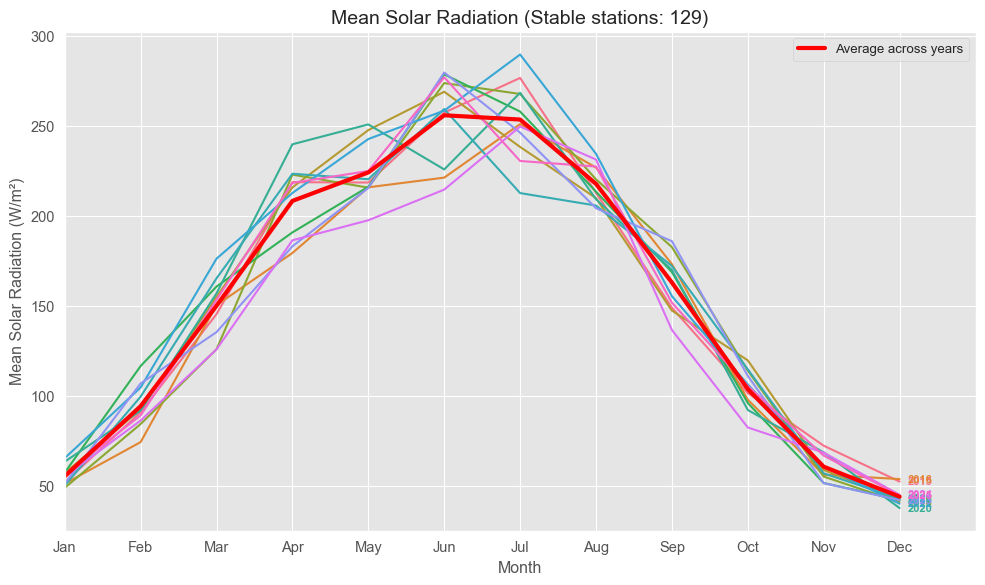
\includegraphics[width=\linewidth]{figures_and_tables/mean_wind_2015_2025.png}
        %\caption{Première image}
    \end{minipage}\hfill
    \begin{minipage}{0.48\textwidth}
        \centering
        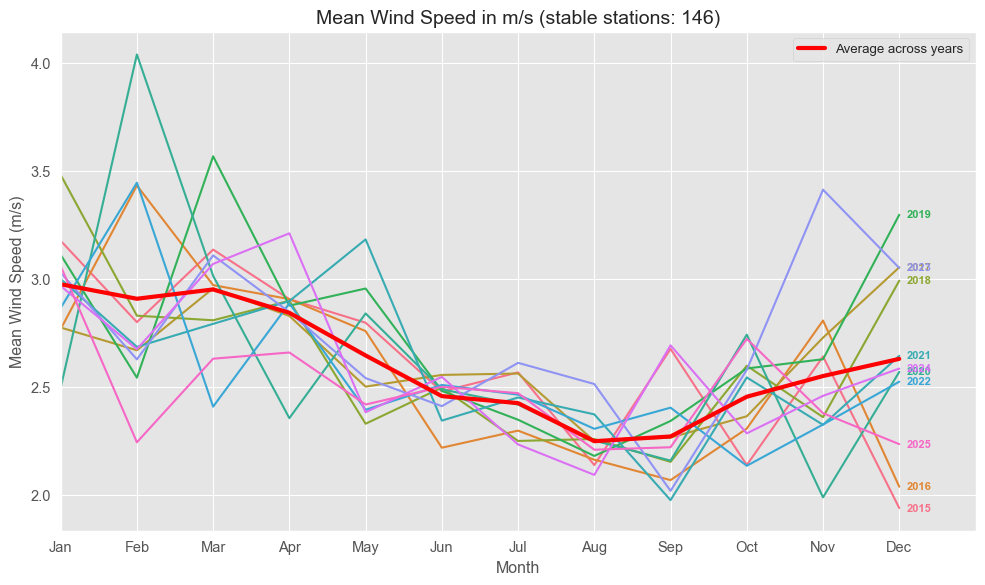
\includegraphics[width=\linewidth]{figures_and_tables/mean_solar_2015_2025.png}
        %\caption{Deuxième image}
    \end{minipage}
    \caption{Mean wind speed and solar radiation from 2015 to 2025.}
    \label{fig:fig_lubin}
\end{figure}


% ## Results we are looking for
% - explain that we will use the data to determine complementarity though data description and correlation analysis. 

We aim here at studying the complementarity between wind speed and solar radiation to account for a potential electricity production complementarity between wind turbines and PVs. We will use correlations criteria as used by \citet{Canales2019} and product descriptive statistics allowing us to analyse such complementarity. These statistics will cover a seasonal analysis, data stratification accounting for elevation and geographic zone using daily and monthly data.

\bibliographystyle{plainnat}
\bibliography{resources}

\end{document}
